%%%%%%%%%%%%%%%%%%%%%%%%%%%%%%%%%%%%%%%%%
% Short Sectioned Assignment
% LaTeX Template
% Version 1.0 (5/5/12)
%
% This template has been downloaded from:
% http://www.LaTeXTemplates.com
%
% Original author:
% Frits Wenneker (http://www.howtotex.com)
%
% License:
% CC BY-NC-SA 3.0 (http://creativecommons.org/licenses/by-nc-sa/3.0/)
%
%%%%%%%%%%%%%%%%%%%%%%%%%%%%%%%%%%%%%%%%%

%----------------------------------------------------------------------------------------
%	PACKAGES AND OTHER DOCUMENT CONFIGURATIONS
%----------------------------------------------------------------------------------------

\documentclass[paper=letter, fontsize=10pt]{scrartcl} % A4 paper and 11pt font size

%\usepackage[T1]{fontenc} % Use 8-bit encoding that has 256 glyphs
%\usepackage{fourier} % Use the Adobe Utopia font for the document - comment this line to return to the LaTeX default
\usepackage[english]{babel} % English language/hyphenation
\usepackage{amsmath,amsfonts,amsthm} % Math packages
\usepackage[hmargin=2.5cm,vmargin=2.5cm]{geometry}
\usepackage{graphicx}
\usepackage{verbatim}
\usepackage{caption}
\usepackage{subcaption}
\usepackage{bm}

%\usepackage{lipsum} % Used for inserting dummy 'Lorem ipsum' text into the template

\usepackage{sectsty} % Allows customizing section commands
%\allsectionsfont{\centering \normalfont\scshape}
\allsectionsfont{\normalsize} 
 % Make all sections centered, the default font and small caps

\usepackage{fancyhdr} % Custom headers and footers
\pagestyle{fancyplain} % Makes all pages in the document conform to the custom headers and footers
\fancyhead{} % No page header - if you want one, create it in the same way as the footers below
\fancyfoot[L]{} % Empty left footer
\fancyfoot[C]{} % Empty center footer
\fancyfoot[R]{\thepage} % Page numbering for right footer
\renewcommand{\headrulewidth}{0pt} % Remove header underlines
\renewcommand{\footrulewidth}{0pt} % Remove footer underlines
\setlength{\headheight}{12pt} % Customize the height of the header

\numberwithin{equation}{section} % Number equations within sections (i.e. 1.1, 1.2, 2.1, 2.2 instead of 1, 2, 3, 4)
\numberwithin{figure}{section} % Number figures within sections (i.e. 1.1, 1.2, 2.1, 2.2 instead of 1, 2, 3, 4)
\numberwithin{table}{section} % Number tables within sections (i.e. 1.1, 1.2, 2.1, 2.2 instead of 1, 2, 3, 4)
\sloppy
\setlength{\parskip}{3pt}
\setlength\parindent{0pt} % Removes all indentation from paragraphs - comment this line for an assignment with lots of text

%----------------------------------------------------------------------------------------
%	TITLE SECTION
%----------------------------------------------------------------------------------------

\newcommand{\horrule}[1]{\rule{\linewidth}{#1}} % Create horizontal rule command with 1 argument of height

\usepackage{xcolor}
\newcommand{\fixme}[1]{\textcolor{red}{\small [~#1~]}}

\title{	
\normalfont \normalsize 
\textsc{ECE5775 High-Level Digital Design Automation, Fall 2017} \\  
School of Electrical Computer Engineering, Cornell University \\ [11pt]% Your university, school and/or department name(s)
\horrule{0.5pt} \\[0.4cm] % Thin top horizontal rule
\large Lab 2: Digit Recognition System (Part 1) \\ % The assignment title
\small Due Wednesday, September 27, 11:59pm
\horrule{0.5pt} \\[0.5cm] % Thick bottom horizontal rule
\vspace{-15ex}}

%\author{Zhiru Zhang} % Your name
%\date{\normalsize\today} % Today's date or a custom date
\date{}

\begin{document}

\maketitle % Print the title
%----------------------------------------------------------------------------------------
%	PROBLEM 1
%----------------------------------------------------------------------------------------
\section{Introduction}

Handwriting recognition refers to the computer's ability to intelligently interpret handwritten inputs and is broadly applied in document processing, signature verification, and bank check clearing. An important step in handwriting recognition is classification, which classifies data into one of a fixed number of classes. In this lab, you will design and implement a handwritten digit recognition system based on the \textbf{k-nearest-neighbors (k-NN)} classifier algorithm \cite{knn}, and eventually implement it on AWS FPGA instance. 

%Specifically, we are provided with 10 sets of already classified handwritten digits (called the training sets), and would like to implement a k-NN algorithm that is able to identify any input handwritten digit (called the testing instance) using the training sets. 
% This assignment is meant to help you build up the necessary foundation for the course project.

In the first part of this lab (this particular assignment), you are provided with a set of already classified handwritten digits (called the training sets), and will implement a k-NN algorithm in C++ that is able to identify any input handwritten digit (called the testing instance) using the training sets. In addition, you will use two commonly-used high-level synthesis (HLS) optimizations to parallelize the synthesized hardware and explore design trade-offs in performance and area. Later in the second part of this lab (Lab 3), you will further optimize the performance of your hardware design and implement the complete digital recognition system on the AWS FPGA instance.

%Please be sure to read the entire assignment carefully before proceeding.

\section{Materials}
\label{materials}

%\begin{enumerate}
%\item

You are given a zip file named 
$lab2.zip$ on $ecelinux$ under $/classes/ece5775/labs$. It contains two directories: \textbf{lab2} and \textbf{harness}. 

\begin{itemize}
	\item \textbf{lab2}: contains all the codes and data of this lab.
	\item \textbf{harness}: contains the wrapper code of OpenCL APIs and top-level makefile. Students are \textbf{not required} to understand the content of this directory.
\end{itemize}
%\item $setup$: a bash script to set up Xilinx tools in your environment. You can either source this script manually per login (. ./$setup$) or add it to your $.bashrc$ file. Note that there are \textbf{two dots} separated by a space in the script sourcing command.

The structure of directory \textbf{lab2} is described as following:

\begin{itemize}
  \item \textbf{src}: 
   	\begin{itemize}
	 	\item \textbf{host}: contains all the codes for host.
		 	\begin{itemize}
	 			\item \texttt{check\_result.cpp}: contains function to print out the errors and calculate the overall error rate.
				\item \texttt{check\_result.h}: the header file of check\_result.cpp.
	 			\item \texttt{digit\_recognition.cpp}: the main file, defines the implementation flow of this application
				\item \texttt{testing\_data.h}: declares two constant arrays including the testing data and corresponding expected labels. 
				\item \texttt{training\_data.h}: combines all the training data sets (i.e., data/testing set.dat) into a constant array. 
				\item \texttt{typedefs.h}: the constant definitions and typedefs for the host. 
				\item \texttt{utils.cpp}: contains the functions to print usage and parse the command line arguments
				\item \texttt{utils.h}: the header file of 
			\end{itemize}
		\item \textbf{ocl}: contains the actual kernel file.
		 	\begin{itemize}
	 			\item \texttt{digitrec.cpp}: \textbf{an incomplete} file that defines the kernel function Digitrec.
			\end{itemize}
	\end{itemize}
  \item \textbf{data}:
  	\begin{itemize}
	 	\item \texttt{training\_set\_\#.dat}: training set for digit $\#$, where $\#=0,1,2,...,9$.
		\item \texttt{testing\_set.dat}: a set of testing instances with corresponding expected labels.
		\item \texttt{expected.dat}: the expected labels of the testing set.
	\end{itemize}
  \item \textbf{makefile}: the makefile to compile the this application.
  \item \textbf{run1.sh}: this script runs the emulation with k value set to 3 by default.
  \item \textbf{run5.sh}: this script runs the application for 5 times with the k value of KNN from 1 to 5.
\end{itemize}


Before starting your assignment, please copy and unzip the zip file to the correct director on your AWS instance, e.g. $\sim/src/project\_data/$ . 


\section{Design Overview}

%The goal of this assignment is to implement a digital recognition design using the k-NN algorithm. 
\textbf{You are given 10 training sets, each of which contains 1800 49-bit training instances for a different digit (0-9). Each hexadecimal string in $training\_set\_\#$ represents a 49-bit training instance for digit $\#$.} 
The 49 bits of each instance encodes a 7x7 matrix of binary values (i.e., a bitmap). For example, \texttt{$e3664d8e00_{16}$} in $training\_set\_0$ is a training instance for digit 0 and translates into the binary 2D matrix in Figure~\ref{fig:zero2d}, whose 1 bits outline the digit 0. A binary image of the array is shown in Figure~\ref{fig:zeroim}. \texttt{$41c0820410_{16}$} in $training\_set\_7$ is a training instance for digit 7 and translates into the binary 2D matrix in Figure~\ref{fig:seven2d}, whose 1 bits approximately outline the digit 7. The corresponding binary image is shown in Figure~\ref{fig:sevenim}. As you can see, the resolution of the digit is limited by the number of bits (49 bits in our assignment) used to represent it. Typically, increasing the number of bits per instance would improve the resolution and possibly the accuracy of recognition. 
%If you like, you may include, as part of your report, discussions on the trade-offs involving the number of bits per instance.

We would like to devise an algorithm that takes in a binary string representing a handwritten digit (i.e. the testing instance) and classify it to a particular digit (0-9) by first identifying $k$ training instances that are closest to the testing instance (i.e., the nearest neighbors), and then determining the result based on the most common digit represented by these nearest neighbors. 

In the latter part of the lab, we would like to research the influence of different choices of k values, and try to analyze the impact and tradeoff of the design choices.

%which digit's training set contains the binary string (i.e. the training instance) that is closest to the testing instance. \textbf{The training set with the training instance that is closest in distance to the testing instance determines the digit that is most likely represented by the testing instance.} 
You are encouraged to read through \cite{knn} to familiarize yourself with the basic concepts of the k-NN algorithm. \textbf{In this assignment, we define the distance between two instances as the number of corresponding bits that are different in the two binary strings.} For example, $1011_2$ and $0111_2$ differ in the two most significant bits and therefore have a distance of 2. $1011_2$ and $1010_2$ differ only in the least significant bit and have a distance of 1. As a result, $1011_2$ is closer to $1010_2$ than to $0111_2$. %An overview of the digital recognition system based on the k-nearest neighbor algorithm is shown in Figure \ref{block}.

\begin{comment}
\texttt{0000000\;\;\;\;\;0000000\\
0011100\;\;\;\;\;0001000\\
0110110\;\;\;\;\;0011100\\
0110010\;\;\;\;\;0000100\\
0110110\;\;\;\;\;0001000\\
0011100\;\;\;\;\;0001000\\
0000000\;\;\;\;\;0010000
}
\end{comment}

\begin{figure}[h]
        \centering
        \begin{subfigure}[b]{0.4\textwidth}
\centering
                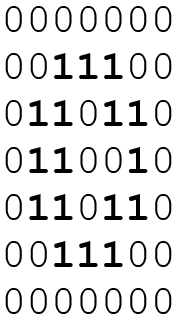
\includegraphics[scale=0.25]{digit0raw.png}
                \caption{Binary string in 2D array}
                \label{fig:zero2d}
        \end{subfigure}%
        ~ %add desired spacing between images, e. g. ~, \quad, \qquad, \hfill etc.
          %(or a blank line to force the subfigure onto a new line)
        \begin{subfigure}[b]{0.4\textwidth}
\centering
                
\includegraphics[trim=1cm 1cm 1cm 1cm, width=0.4\textwidth]{digit0.png}
                \caption{Binary image}
                \label{fig:zeroim}
        \end{subfigure}
\caption{Training instance for digit 0}
\end{figure}

        ~ %add desired spacing between images, e. g. ~, \quad, \qquad, \hfill etc.
          %(or a blank line to force the subfigure onto a new line)
\begin{figure}[h]
        \centering 
       \begin{subfigure}[b]{0.4\textwidth}
\centering
                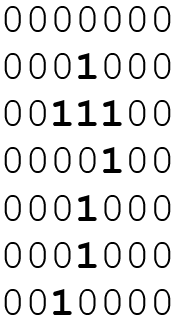
\includegraphics[scale=0.25]{digit7raw.png}
                \caption{Binary string in 2D array}
                \label{fig:seven2d}
        \end{subfigure}
\begin{subfigure}[b]{0.4\textwidth}
\centering
                
\includegraphics[trim=1cm 1cm 1cm 1cm, width=0.4\textwidth]{digit7.png}
                \caption{Binary image}
                \label{fig:sevenim}
        \end{subfigure}
        \caption{Training instance for digit 7}\label{fig:animals}
\end{figure}
%\begin{figure}[]
%  \centering
%  \includegraphics[width=0.9\textwidth]{digit_block_diagram.png}
%  \caption{Digit recognition block diagram (will be replace)}
%  \label{block}
%\end{figure}
\begin{comment}
\begin{itemize}
\item \textit{nearest\_neighbor} iterates through all training sets (\textit{training\_set\_0} to \textit{training\_set\_9}). For each training set, it determines the minimum distance between the input handwritten digit and any piece of training data in the set. \footnote{The training set for each digit consists of one piece of training data per line.}  The digit whose training set results in the minimum distance is the digit that is recognized.
\item \textit{find\_min\_difference} iterates through all pieces of data within a particular training set (for example $0xe3664d8e00$ to $0x71e6cd9e00$ in \text{training\_set\_0}) and find the minimum distance between its input handwritten digit and any piece of data in the training set.
\item \textit{find\_difference} computes the bitwise XOR between its two inputs.
\item \textit{count\_set\_bits} computes the number of bits in the input that are 1's.
\end{itemize}

As shown in the block digram, there is a hierarchical dependence between the different blocks. \textit{nearest\_neighbor} depends on \textit{find\_min\_difference} to determine the input's minimum distance with each digit's training set. \textit{find\_min\_difference} uses \textit{find\_difference} to compute the distance between two pieces of data. \textit{find\_difference} needs \textit{count\_set\_bits} to count the number of 1's in the XOR result in order to quantify the distance.
\end{comment}

\section{Guidelines and Hints}

\subsection{Coding and Debugging}
%The first part of this assignment is to implement a functional digit recognition core as your baseline design. 

Your first task is to complete the digit recognition algorithm based on the code skeleton provided in $src/ocl/digitrec.cpp$. 
%Your \textit{nearest\_neighbor} function should iterate through the 10 training sets and find the training set $S$ that contains the training instance that is closest in distance to the testing instance. The function then returns the digit corresponding to the specific training set $S$.
%If you like, you may consider implementing the design hierarchically by defining and calling the following helper functions.
In particular, you are expected to fill in the code for the following functions:
\begin{itemize}
\item \textit{update\_knn}: Given the testing instance and a (new) training instance, this function maintains/updates an array of $k$ minimum distances per training set.
\item \textit{knn\_vote}: Among $10 \times k$ minimum distance values, this function finds the $k$ nearest neighbors and determines the final output based on the most common digit represented by these nearest neighbors.
\end{itemize}

Note that the skeleton code takes advantage of arbitrary precision integer type \textit{ap\_uint}. \textbf{A useful reference of arbitrary precision integer data types can be found on p.620--638 of the user guide~\cite{ug902} (please pay special attention to the bitwise and bit selection operations).}

How you choose to implement the algorithm may affect the resulting accuracy of your design as reported by the test bench. \textbf{We expect that your design would achieve an error of less than 10\% on the provided testing set.} You may use the console output or the generated $out.dat$ file to debug your code.

Be aware that a bash script \textit{run1.sh} is provided for you to run the software emulation, the k value is set to 3 by default, and you can specify the k value in the script. You can run the script with $./run1.sh$

\subsection{Design Exploration}
\label{design-expl}
The second part of the assignment is to explore the impact of the $k$ value on your digit recognition design. Specifically, \textbf{you are expected to experiment with the $k$ values ranging from 1 through 5, and collect the performance and area numbers of the synthesized design for each specific $k$.} 

    The actual $k$ value can be specified in $run5.sh$. You can run the software emulation in batch with $./run5.sh$. This script will also automatically collect the 5 estimation reports and combine them in a single file under $results$ folder. You are going to look into the stats to analyze the impact of different k values.
    %This script will also automatically collect important stats (i.e., accuracy, performance, and resource usage) from the Vivado HLS reports and generate a $knn\_result.csv$ file under the $result$ folder.
  

\subsection{Design Optimization}
\label{design-opt}
The third part of the assignment is to optimize the design with HLS pragmas or directives. In particular, we will focus on exploring the effect of the following optimizations in our design and apply them appropriately to \textbf{minimize the latency of the synthesized design (Hint: the final optimized latency should be roughly one order of magnitude lower than the baseline you obtained from experimentation described in Section~\ref{design-expl}).} 
\begin{itemize}
\item \textbf{loop unrolling} unfolds a loop by creating multiple copies of its loop body and reducing its trip count accordingly. This technique is often used to achieve shorter latency when loop iterations can be executed in parallel. 
%\item \textbf{loop pipelining}: enables the loop to process a new iteration every II clock cycles, where II is the initiation interval.
\item \textbf{array partitioning} partitions an array into smaller arrays, which may result in an RTL with multiple small memories or multiple registers instead of one large memory. This effectively increases the amount of read and write ports for the storage.
\end{itemize}

Please refer to the following user guide for details on how to apply these optimization using Vivado HLS (v2016.2). 

\begin{itemize}
\item Vivado Design Suite User Guide, High-Level Synthesis, UG902 (v2016.2)~\cite{ug902}
\begin{itemize}
%\item \textit{set\_directive\_pipeline} p.462
\item \textit{set\_directive\_unroll} p.481
\item \textit{set\_directive\_array\_partition} p.447
\end{itemize}
You may insert pragmas or set directives to apply these optimizations. You can find code snippets with inserted pragmas throughout the user guide (e.g. p.146, p.151).
\end{itemize}

\textbf{Other than the added pragmas/directives, your program should look the same with baseline.}

In this experiment, please avoid unrolling the outermost loop (i.e., the one that iterate 1800 times) so your design would not require excessive chip area. Also for the sake of simplicity, please try to only use fixed-bound $for$ loop(s) in your program. Note that $while$ loops are synthesizable but may lead to a variable-latency design that would  complicate your reporting. \footnote{You will need to enable C-RTL co-simulation to get the actual cycle count for a design with data-dependent loop bounds.} 

\subsection{Report}
(not updated yet, will be updated after the previous parts are settled)
\begin{itemize}
\item Please write your report in a \textbf{single-column and single-space format with a 10pt font size. Page limit is 2. Please include your name and NetID on your report.}

\item The report should start with an overview of the document. This should inform the reader what the report is about, and highlight the major results. In other words, this is similar to an abstract in a technical document. Likewise there should be a summary, describing the results, and highlight the important points.
%\item The report should include a module-level block diagram of the datapath of the synthesized design. This means that you can treat each module as a black box and simply include the interface of each module (by drawing the RTL ports that are also in your C/C++ implementation). Please also clearly indicate the optimization(s) applied in each module. \textbf{The synthesis report should contain enough details on the synthesized modules to help you with your block diagram.}

\item There should be a section describing how you implement the $update\_knn$ and $knn\_vote$ functions.

\item There should be a section comparing different $k$ values with a table that summarizes the key stats including the error rate (accuracy), area in terms of resource utilization (number of BRAMs, DSP48s, LUTs, and FFs), and and performance in latency in number of clock cycles.\footnote{Check out the synthesis report under $knn.prj/solution1/syn/report/$.} 

\item There should be a section describing how you would add the HLS pragmas/directives to minimize the latency of the synthesized design. Please contrast the performance and area of your most optimized design (i.e., with smallest latency) with the baseline design. For this comparison, you only need to set $k$ to 3. 

%The document should be written in complete sentences - no fragments or just a bunch of bullet points (some bullet points are fine, but this should not be the entire document).

%	\item All of the figures and tables should have captions. These captions should do their best to completely explain the figure (explain axis, units, etc.). Ideally you can understand the report just by looking at the figures and captions. But please avoid just putting some results and never saying anything about them.

\item Showing small snippets of your code to show the use of pragmas or to demonstrate the restructuring of the code is fine, but please avoid listing every single line of the code every optimization. It is possible to be succinct and thorough at the same time.

\item The report should only show screenshots from the tool when they demonstrate some significant idea. If you do use screenshots, make sure they are readable (e.g., not blurry). In general, you are expected to create your own figures. While more time consuming, it allows you to show the exact results, figures, and ideas you wish to present.

%	\item Please think about the best way to plot the results. For example, bar graph vs. line graph, or Log vs. linear scale on the axis.Please avoid plotting a lot of random data without providing insights. (Hint: if it is hard to explain, then you should rethink about what you are presenting, i.e., organize the data in a different way.)
\end{itemize}

\section{Deliverables}
\label{deliverables}
\textbf{Please submit your assignment on CMS.} You are expected to submit your report and your code and scripts (and only these files, not the project files generated by the tool) in a zipped file named \textbf{digitrec.zip} that contains the following contents:
\begin{itemize}
	\item $report.pdf$: the project report in pdf.
    \item A folder named $solution$: the set of source files and scripts required to reproduce your experiments (including the pragams/directives for design optimization).  
    Note that only these files should be submitted. Please run $make$ $clean$ to remove all the automatically generated output files. 
\end{itemize}

% This means that you should either use pragmas in your code or include the Tcl script with the optimization directives.

\section{Acknowledgement}
This design originated from an ECE-5775 project originally implemented by Ackerley Tng and Edgar Munoz. 

\begin{thebibliography}{3}
\bibitem{knn}

Kun, Jeremy. \emph{K-Nearest-Neighbors and Handwritten Digit Classification}. Math Programming. Available at https://jeremykun.com/2012/08/26/k-nearest-neighbors-and-handwritten-digit-classification
\bibitem{ug902}
Xilinx Inc. \emph{Vivado Design Suite User Guide: High-Level Synthesis UG902 (v2016.1)},
Available at http://www.xilinx.com/support/documentation/sw\_manuals/xilinx2016\_2/ug902-vivado-high-level-synthesis.pdf
%\bibitem{guide}
%  Xilinx Inc. \emph{Introduction to FPGA Design with Vivado High-Level Synthesis}. 2013.

\end{thebibliography}

\end{document}
